\documentclass{beamer}
%\usetheme[footline=infoline,headline=secheader]{UPB}
%\usetheme[footline=infoline,headline=structure]{UPB}
%\usetheme[headline=secheader]{UPB}
%\usetheme[headline=structure]{UPB}
%\usetheme[footline=infoline]{UPB}
%\usetheme{UPB} % defaults are footline=empty,headline=empty
%\usetheme{Antibes}
%\usetheme{upb}
\setbeamertemplate{bibliography item}[text]
\author[C.Robbert, P. Stilow]{Christoph Robbert, Peter Stilow}
\institute[Uni Paderborn]{Universität Paderborn}

\title[Protokoll 0/Aufgabe 1]{Protokoll 0/Aufgabe 1}
\begin{document}
\begin{frame}
\maketitle
\end{frame}

\begin{frame}
\begin{figure}
	\label{0_netlayout}
	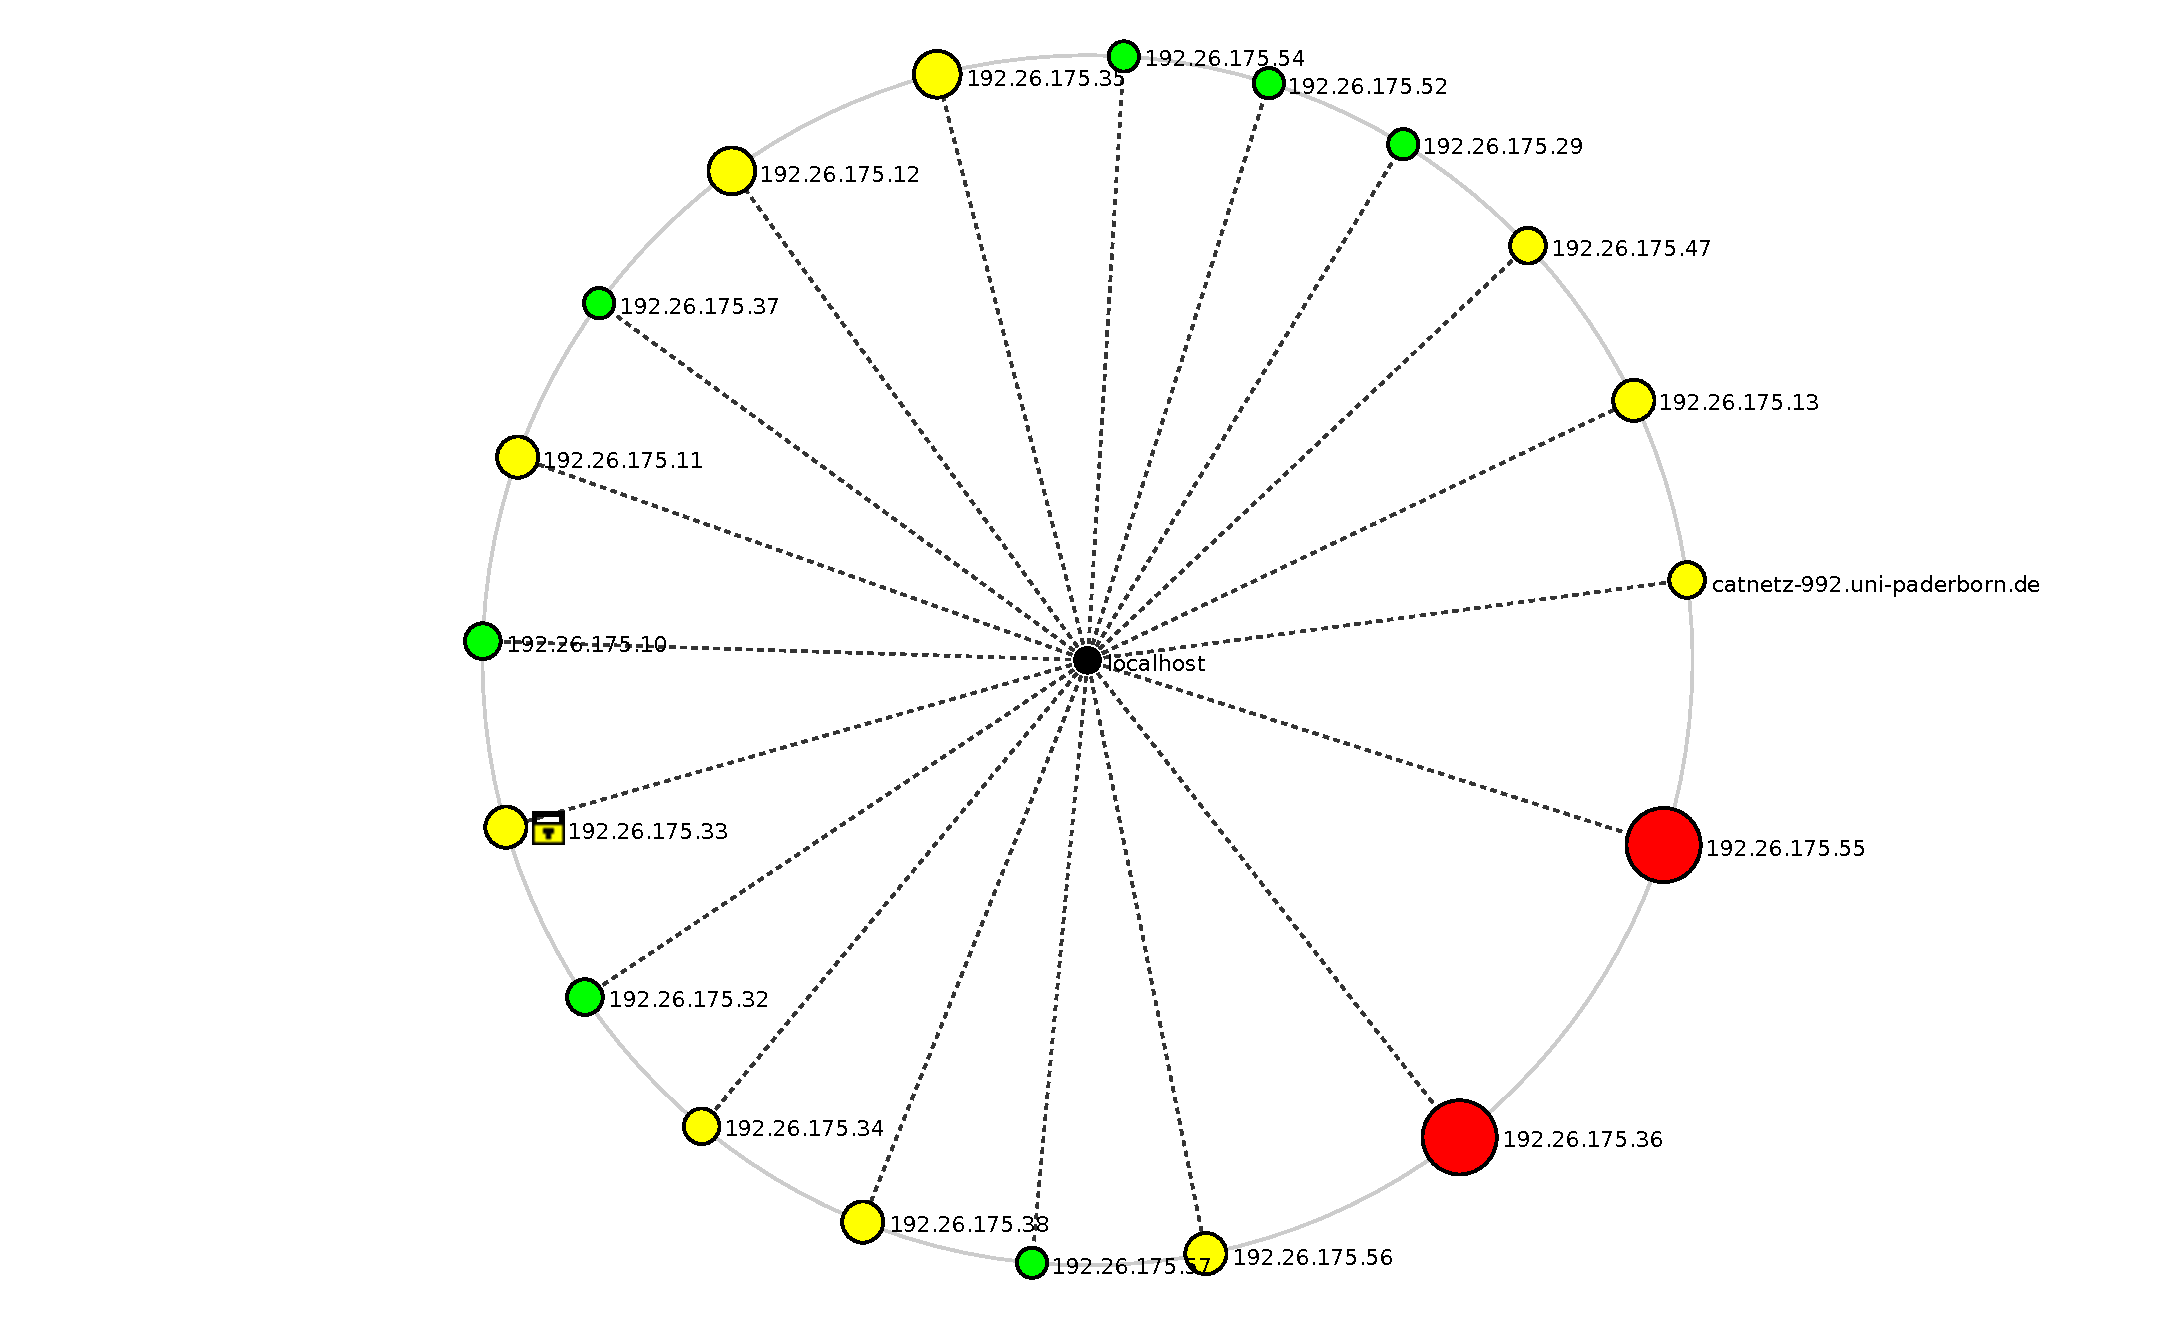
\includegraphics[scale=0.3]{figures/0_netlayout.pdf}
	\caption{Struktur des Netzes im Security Lab. Localhost ist unser Laptop, der für die Scans benutzt wurde. Zenmapgrafik für Kommando: \texttt{nmap -sP 192.26.175.0/26}}
\end{figure}
\end{frame}

\begin{frame}[fragile]
Portscan \texttt{nmap -sT -sV 192.26.175.10}
\begin{footnotesize}
	\begin{verbatim}
22/tcp  open  ssh     OpenSSH 5.9p1 Debian 5ubuntu1 (protocol 2.0)
111/tcp open  rpcbind
Service Info: OS: Linux
	\end{verbatim}
\end{footnotesize}

\end{frame}


\begin{frame}[fragile]
Portscan \texttt{nmap -sT -sV 192.26.175.29}
\begin{footnotesize}
	\begin{verbatim}
139/tcp open  netbios-ssn
137/udp open|filtered netbios-ns
138/udp open|filtered netbios-dgm
	\end{verbatim}
\end{footnotesize}

\end{frame}

\begin{frame}[fragile]
Portscan \texttt{nmap -sT -sV 192.26.175.29}
\begin{footnotesize}
\begin{verbatim}
7/tcp    open  echo
9/tcp    open  discard?
13/tcp   open  daytime       Microsoft Windows USA daytime
17/tcp   open  qotd          Windows qotd (English)
19/tcp   open  chargen
21/tcp   open  ftp           Microsoft ftpd
25/tcp   open  smtp          Microsoft ESMTP 6.0.3790.3959
135/tcp  open  msrpc         Microsoft Windows RPC
139/tcp  open  netbios-ssn
445/tcp  open  microsoft-ds  Microsoft Windows 2003 or 2008 microsoft-ds
548/tcp  open  afp?
1025/tcp open  msrpc         Microsoft Windows RPC
1028/tcp open  msrpc         Microsoft Windows RPC
1029/tcp open  msrpc         Microsoft Windows RPC
1030/tcp open  msrpc         Microsoft Windows RPC
3389/tcp open  ms-wbt-server Microsoft Terminal Service
8099/tcp open  http          Microsoft IIS httpd 6.0
Service Info: Host: w2k3; OS: Windows; CPE: cpe:/o:microsoft:windows
\end{verbatim}
\end{footnotesize}

\end{frame}
\end{document}